% Template for ICASSP-2020 paper; to be used with:
%          spconf.sty  - ICASSP/ICIP LaTeX style file, and
%          IEEEbib.bst - IEEE bibliography style file.
% --------------------------------------------------------------------------
\documentclass{article}
\usepackage{spconf,amsmath,graphicx, hyperref}

% Example definitions.
% --------------------
\def\x{{\mathbf x}}
\def\L{{\cal L}}

% Title.
% ------
\title{IMPLEMENTING AN OBJECTIVE FUNCTION AND REPORTING THE EFFECTS OF REGULARISATION ON GENERATIVE MODELS}
%
% Single address.
% ---------------
\name{Chad Kakau \thanks{AIML425}}
\address{Victoria University, Wellington}
%
%
\begin{document}
%\ninept
%
\maketitle
%
\begin{abstract}
This paper revises the concept of objective functions as applied in machine learning and identifies the Maximum Mean Discrepency used by the author in the implementation of a generative neural network.  The generative model maps a gaussian distribution to a uniform distribution, then maps the uniform distribution to a gaussian distribution, for a concatenated gaussian to gaussian network.  This paper briefly describes the intuition behind the Maximum Mean Discrepency, and implements the method with three levels of L2 regularisation.  Best performance occurs with $L2 = 1e^{-6}$, but at all levels of L2, the second half of the network tends to train toward higher positive values, rather than a normal distribution.  This is most likely the result of implementation issues.  
\end{abstract}
%
\begin{keywords}
objective function, maximum mean discrepancy, kernel
\end{keywords}
%
\section{Introduction}
\label{sec:intro}
%
Neural networks have become a mainstay of image processing over the last two decades (compare \cite{parisi1998car} and \cite{naranjo2020review}).  Regularly employing stochastic gradient descent, supervised training of neural networks involves driving an algorithm towards a target classification or probability distribution by minimising the distance between the actual class/distribution and the prediction \cite{samek2021explaining}.  This paper implements the Maximum Mean Discrepancy method to, ultimately, produce a Gaussian Process, which should result in a Gaussian distribution as an output \cite{Rasmussen2004}.  Thus, the expected outcome of this implementation should be a 2D Gaussian distribution, which, given the same scale between the two output variates, should produce a circular plot.    

\section{Objective function and kernel}
\label{sec:format}

We train a neural network using stochastic gradient descent so that it can iteratively learn and adjust from the prediction (based on each instance, or input vector) and distance from the actual target (output vector).  One of the main decisions for the design of the network is the selection of an objective function to drive the model predictions toward the target.  Although numerous objective functions are possible, this implementation uses the Maximum Mean Discrepancy which measures the distance between two distributions.  For optimisation the model aims to minimise MMD.  Before working through the theory of the MMD, we need to first briefly discuss the kernel - a concept which has taken several days of bashing my head against the internet wall, for me to finally come to grips with.  

\subsection{The kernel function reduces the complexity of calculation without sacrificing detail}
\label{ssec:kernel}

After several lectures, reviews of lecturs, scanning of the internet and multiple re-visits to wikipedia, I think the kernel, is a matrix that transforms our input vector in a lower dimensional space to the dot product output vector in a higher dimensional space \cite{wilimitis_2019} \cite{hofmann2008kernel}.  I struggled alot with the concept of the kernel, because I didn't take the time to look up what an inner product means... it turns out, an inner product is the result of multiplying two vectors and resolves to a scalar value.  The kernel provides a mechanism for plotting data that is not linearly separable in lower dimensions, into higher dimensions where they can be separated by a linear function.  

\subsection{Maximum Mean Distribution as the objective function}
\label{ssec:mmd}

With the distribution $p_Y$ as:  

$\frac {1}{n(n-1)}\sum_{i\ne j} k(y^{(i)}, y^{(j)})$  

and $p_X$ as:   

$\frac {1}{m(m-1)}\sum_{i\ne j} k(x^{(i)}, x^{(j)})$,  

where $k(x, y)$ is a positive definite kernel (in this case, the Gaussian
kernel) then intuitively, if the distributions are the same then adding the two together should equate to their joint distribution:  

$$
\begin {aligned}
MMD&(\{x^{(i)}\}_{i=1, ..., m}, \{y^{(j)}\}_{j=1, ..., n}) \\
  & = \frac {1}{n(n-1)}\sum_{i\ne j} k(y^{(i)}, y^{(j)}) 
  + \frac {1}{m(m-1)}\sum_{i\ne j} k(x^{(i)}, x^{(j)}) \\
  & - 2\frac{1}{mn}\sum_{i,j}k(x^{(i)},y^{(j)})
\end {aligned}
$$
%
We can take advantage of the reproducing nature of the Gaussian kernel to reduce the MMD comparing the sum of the mean-squares of the two individual distributions, against the 2 times the mean-square of the joint distribution. 

\section{RESULTS}
\label{sec:results}
%
The results show that training a network to learn a Gaussian to Uniform distribution is fairly successful, evidenced by the similarity between the target data and the test data for the first part of the training.  Some of the learned network projects outside of the target area (i.e. greater than 1), which is likely an error in the transformation math (i.e. no epxlicit constraint placed on the output of the $f_1$ network.  Training the network from uniform to Gaussian was less successful, resulting in a skewed dataset with a high proportion of datapoints near the mean, but not is equally spread as the training data.  


\begin{figure}[htb]

\begin{minipage}[b]{1\linewidth}
  \centering
  \centerline{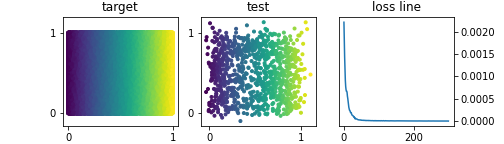
\includegraphics[width=8.5cm]{f1_0.01_300_1000}}
%  \vspace{2.0cm}
\end{minipage}
%  \vspace{2.0cm}
\begin{minipage}[b]{1\linewidth}
  \centering
  \centerline{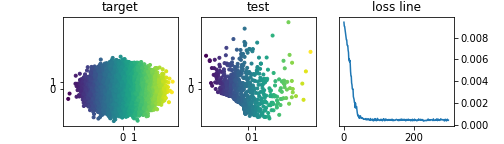
\includegraphics[width=8.5cm]{f2a_0.01_300_1000}}
%  \vspace{2.0cm}
\end{minipage}
%
\caption{$f_1$ and $f_{2a}: L2 = 1e^{-2}$}
\label{fig:res}
%
\end{figure}

There is a difference between regularisation values at $L2 = {1e^{-6}, 1e^{-2}, 1}$, but it is diffiult to discern from the plots.  Best performance across both networks ($f_1$ an $f_{2a}$) was achieved with $L2 = 1e^{-6}$, followed by $L2 = 1e^{-2}$ and then $L2 = 1$.  

\begin{figure}[htb]
\begin{minipage}[b]{1\linewidth}
  \centering
  \centerline{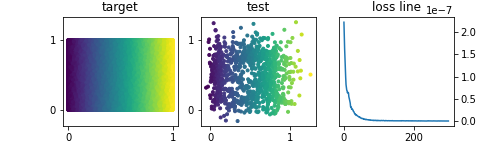
\includegraphics[width=8.5cm]{f1_1e-06_300_1000}}
%  \vspace{1.5cm}
\end{minipage}
%
\begin{minipage}[b]{1\linewidth}
  \centering
  \centerline{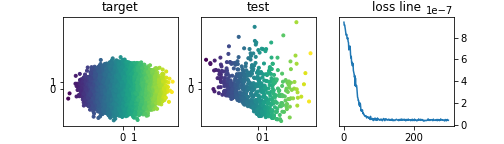
\includegraphics[width=8.5cm]{f2a_1e-06_300_1000}}
%  \vspace{1.5cm}
\end{minipage}
%
\caption{$f_1$ and $f_{2a}$, $L2 = 1e^{-6}$}
\label{fig:res1}
%
\end{figure}
When $L2 = 0.01$, the $f_1$ network trains well, with good spread of data, mostly contained within the bounds of 0 and 1 (Fig \ref{fig:res}).  The $f_{2a}$ network doesn't learn so well, the input data forming a two orthogonal, normal distributions, but the test output fails to train so well, with strong centralisation of data and a general tendency towards positive values.

When $L2 = 1e^{-6}$, the $f_1$ network again trains well, with good spread of data, mostly contained within the bounds of 0 and 1 (Fig \ref{fig:res1}).  The $f_{2a}$ network doesn't learn so well, the input data forming two orthogonal, normal distributions, but the test output again tends toward positive values.

When $L2 = 1$, both the $f_1$ and $f_{2a}$ networks both train and deliver similar outputs as with previous levels of L2 regularisation, however, performance is not as good, with loss, predictably 2 orders of magnitude higher than when $L2 = 1e^{-2}$ (Fig \ref{fig:res2}).

\begin{figure}[htb]
\begin{minipage}[b]{1\linewidth}
  \centering
  \centerline{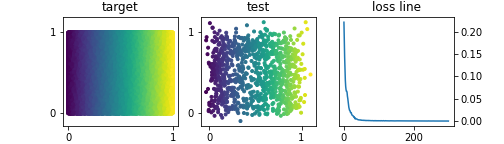
\includegraphics[width=8.5cm]{f1_1_300_1000}}
%  \vspace{1.5cm}
\end{minipage}
%
\begin{minipage}[b]{1\linewidth}
  \centering
  \centerline{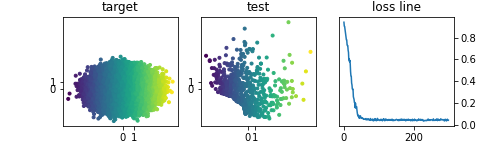
\includegraphics[width=8.5cm]{f2a_1_300_1000}}
%  \vspace{1.5cm}
\end{minipage}
%
\caption{$f_1$ and $f_{2a}$, $L2 = 1$}
\label{fig:res2}

\end{figure}

\hfill



\section{CONCLUSION}
\label{sec:CONC}

The results of the implementation are inconsistent with the expected outcome - the Gaussian to Uniform to Gaussian transformation should maintain relatively stable and consistent distributions between input and output.  The central uniform distribution provides for a consistent and predictable target so that concatenation can move in either direction.  The most likely cause is poor implementation, in either the application of the L2 regularisation function, the application of the kernel function, or the definition of the objective function.  
The L2 regularisation was applied at the loss function, with a simple multiplication of the mean-squared error.  The loss function itself was the mean-squared error (for both $f_1$ and $f_{2a}$ networks).  The kernel function was not explicitly applied.  Future implementations should develop specific models for each phase of the transformation (i.e. $f_1$ and $f_{2a}$).

Link to colab site for code: 

\url{https://colab.research.google.com/drive/1PvCfr1n0tMmiZp878WpvcSFX9GwWINXI?usp=sharing}

\bibliographystyle{IEEEbib}
\bibliography{refs}

\end{document}
